%!TEX root = ../../report.tex
\section{Probability Input  Markov Chain}
\label{sec:pmac}
The comparison between IMAC and HMM in figure \ref{fig:markow_learning} shows that incorporating the noise in the learning method has benefits. The HMM approaches the correct value as more observations are added. The HMM learning is slow at converging on a value, unlike IMAC. When there is no noise the IMAC is an excellent solution. 

\subsection{Developing on Independent Markov Chains}
The IMAC method considers an observation to be either occupied or free. However, in the system setup used in this project the input is the probability for a cell being occupied. To use IMAC it is necessary to determine the state of the observation with one or two thresholds. The simplest choice is placing a threshold at $0.5$ rendering everything above as an occupied observation and everything below a free. This approach will make no distinction between an observation of $0.501$ and $0.999$, which both will be considered occupied and contribute equally in the learning process. This is not desirable as the latter measurement contains immensely more information than the former. 

Equating all measurements on the basis that they fall on the same side of a threshold reduces the advantage of taking position and sensor noise into consideration with the static mapper. 
It is problematic if a cell is observed with low uncertainty and later with a high uncertainty. 
These two entries into the IMAC learner considered equally important.
If for instance a reading resulted in $0.99$ occupancy probability and the following reading produced $0.49$ occupancy probability, the simple threshold method would register it as an occupied followed by a free and thus adding an event. 
In reality there is little evidence for this event happening and if the subsequent reading produces $0.99$ occupancy probability this would introduce even more dynamics regardless of the inconclusive evidence. 
Therefore a method to incorporate the uncertainty in observations and carrying them into the learner is desired. 
As IMAC is a fast learner of Markov transition probabilities when the observations are very certain, the incorporation of the uncertainties should not hinder this. 

The requirements for the incorporation of the uncertainties are:
\begin{enumerate}
	\item Perform as IMAC on perfect input
	\item Avoid low confidence observations counting as much as high confidence ones
	\item Avoid biasing state transition probabilities
\end{enumerate}

\subsection{Propagation of Uncertainties with PMAC}
The method devised to accomplish the integration of uncertainties is denoted Probability input Markov Chain (PMAC). 
As opposed to IMAC the PMAC uses a score rather than counting observations in a state and events as shown in equation \ref{eq:imac_general} and \ref{eq:pmac_lambda}. 

\begin{equation}
\lambda_{IMAC} = \frac{\#events + 1}{\#observations\; in\; state + 1}
\label{eq:imac_general}
\end{equation}

\begin{equation}
\lambda_{PMAC} = \frac{\Sigma e_{score}}{\Sigma s_{score}}
\label{eq:pmac_lambda}
\end{equation}

The state score is calculated with equation \ref{eq:state_score} for the active state which is determined by whether \(p_{occ} > 0.5\) or not. This ensures that if the reading is certain, i.e. either zero or one the update will be similar to that of IMAC, and as uncertainty increases the score linearly decreases.

\begin{equation}
s_{score}(t)=2 \cdot \left\|0.5-p_{occ}(t)\right\|
\label{eq:state_score}
\end{equation}

Another possible scoring could be the probability for occupied $(p_{occ})$ and free $(1-p_{occ})$.
With this scoring system the denominator in equation \ref{eq:pmac_lambda}  would always be increased with a value of at least $0.5$.
This is due to the switch in active state at $p_{occ} = 0.5$. When $p_{occ} > 0.5$ the state score is equal to $p_{occ}$. Alternatively the score is $(1-p_{occ})$.
This would bias the results of the learning with unknown observations.
The chosen score better incorporates $0.5$ denoting unknown, thus producing a score of $0$.

The event score depends on the certainty for being in the previous and current state. 
The certainty of the current state is modeled by the sum of consecutive state scores while being in the state. This value is denoted $\psi$ in equation \ref{eq:event_score}.
The event score is limited to the average of the consecutive observations in the previous opposite state $\hat{\mu}_{s}$. 
This is done in order to avoid biasing towards dynamic.
As the average cannot exceed one, it ensures that in perfect certainty the behavior is equal to that of IMAC. 
If, instead, the sum had been used, a series of low confidence observations could skew the result. 
As the sum of state scores can be considered $\hat{\mu}_s \cdot n_{obs}$ the event score will be balanced when using $\hat{\mu}_s$ as a maximum value. 
For instance $5$ observation with an occupancy probability of $0.6$ would each give a score of $0.2$, and the sum would consequently be $1$. 
Using the sum,  would be $1/1$  thus skewing it towards dynamics. Using the average, the event score is balanced to the state score and produces a more correct value of $0.2/1$. 
The correctness of this result is evident from the fact that simply counting events and states with IMAC also results in a probability on $\lambda = 1/5$. 
Hence the correct dynamics is estimated with PMAC and the parameters are only updated according to the confidence in the used observations.

\begin{equation}
e_{score}(t)=min(\hat{\mu}_{s},\psi)
\label{eq:event_score}
\end{equation}

Both the state and event score behave as IMAC counters when the certainty is perfect, thus fulfilling the first requirement. The second requirement is achieved by the state score scaling with the occupancy probability distance from $0.5$, and the event score basing its value on the state score.
In order to handle multiple uncertain observations as shown in figure \ref{fig:pmac_noise_problem_case} the $\hat{\mu}_s$ is not only controlled by the average of the previous sum of consecutive state scores of the opposite state, but also a long term average of that state.
This avoids under estimating $\lambda$ in cases with multiple very uncertain values, as demonstrated by figure \ref{fig:pmac_noise_problem_case} and \ref{fig:visualization_of_advantage_long_term_average}.
For a detailed description of PMAC the pseudocode is available in appendix \ref{appendix:pmac_pseudo_code}.

\begin{figure}[htbp]
    \centering
    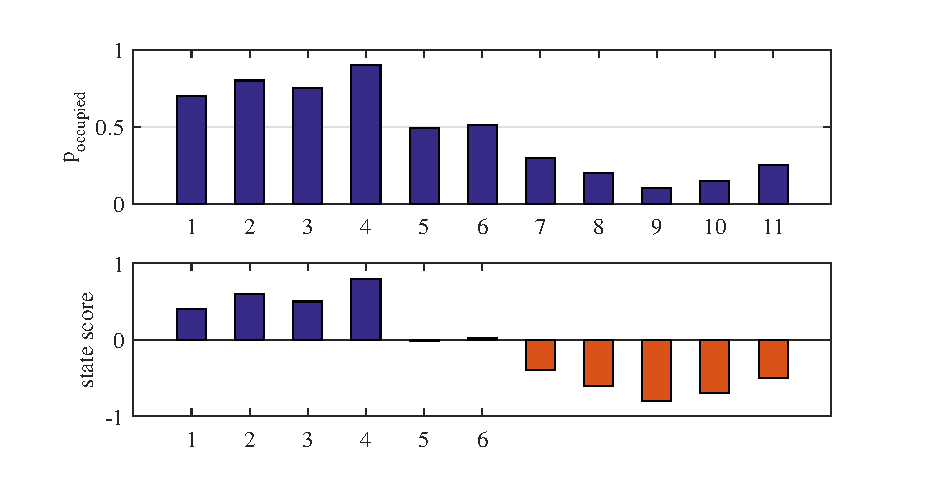
\includegraphics[scale=1]{chapters/mapping_of_dynamic_areas/figures/pmac_noise_problem_case}
    \caption{}
    \label{fig:pmac_noise_problem_case}
\end{figure}


\begin{figure}[htbp]
    \centering
    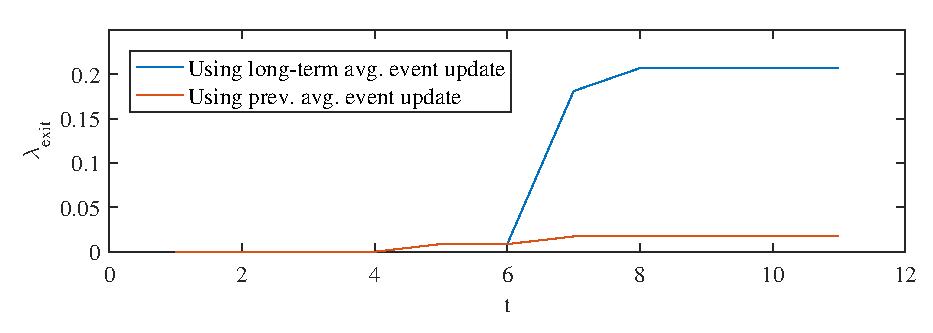
\includegraphics[scale=1]{chapters/mapping_of_dynamic_areas/figures/visualization_of_advantage_long_term_average}
    \caption{}
    \label{fig:visualization_of_advantage_long_term_average}
\end{figure}

\subsection{Case Studies}
The PMAC learning method is illustrated through a couple of case scenarios in the following. 
Figure \ref{fig:state_scores_explained} shows an example of some observations, their occupancy probabilities $p_{occ}$ and the resulting state score $s_{score}$. On the score plot the average of sequential observations in the same state are shown as green lines. This sets a maximum limit on the size of the subsequent event score. To demonstrate the workings of PMAC these observations are used as input to the PMAC learner in the following. 

\begin{figure} [htbp]
    \centering
    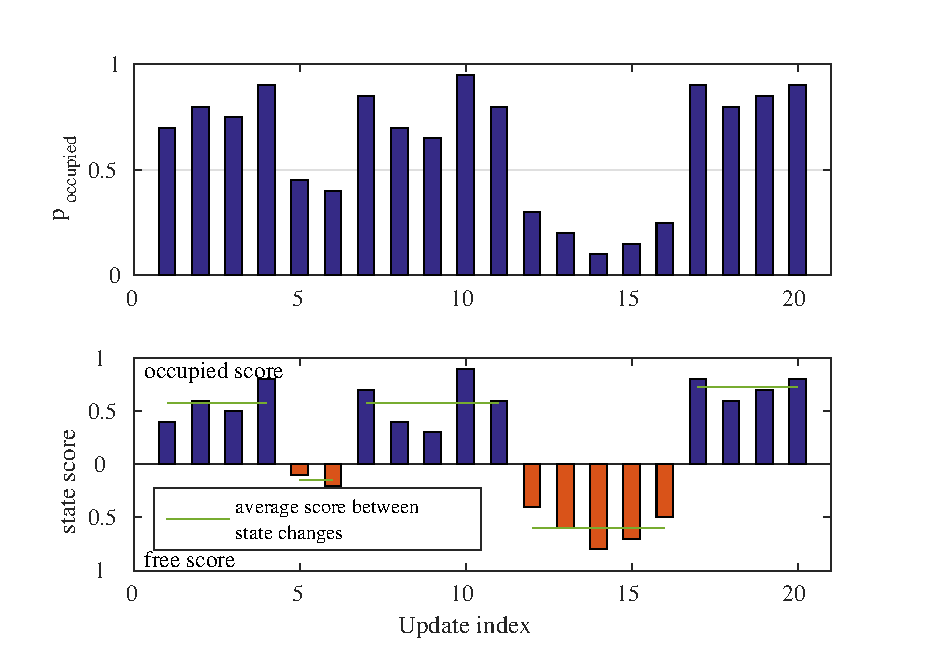
\includegraphics[scale=1]{chapters/mapping_of_dynamic_areas/figures/state_scores_explained}
    \caption{Artificial example of occupancy probabilities used to learn dynamics.}
    \label{fig:state_scores_explained}
\end{figure}

From the state scores in figure \ref{fig:state_scores_explained} it is seen that from index 0 to 11, the situation starts as occupied with quite confident readings. Then two more uncertain readings showing free occurs before confident readings of occupied are again received. The effect of this on the exit is shown in figure \ref{fig:pmac_exit_explained}. The sum of occupied scores increases steadily from index $0$ to $11$, while the event sum increases a comparatively small amount. However it is clearly visible on the exit value as it is the first observations and both sums are initialized to the smallest possible non-zero value. This initialization is chosen in order to avoid dividing by zero and minimizing the effect of initialization. The effects of this initialization is clearly visible in figure \ref{fig:pmac_entry_explained}, that shows the scores and values for the entry. The entry value is one, as the initial values causes, but as soon as input is received their effect is suppressed.

\begin{figure}[htbp]
\centering
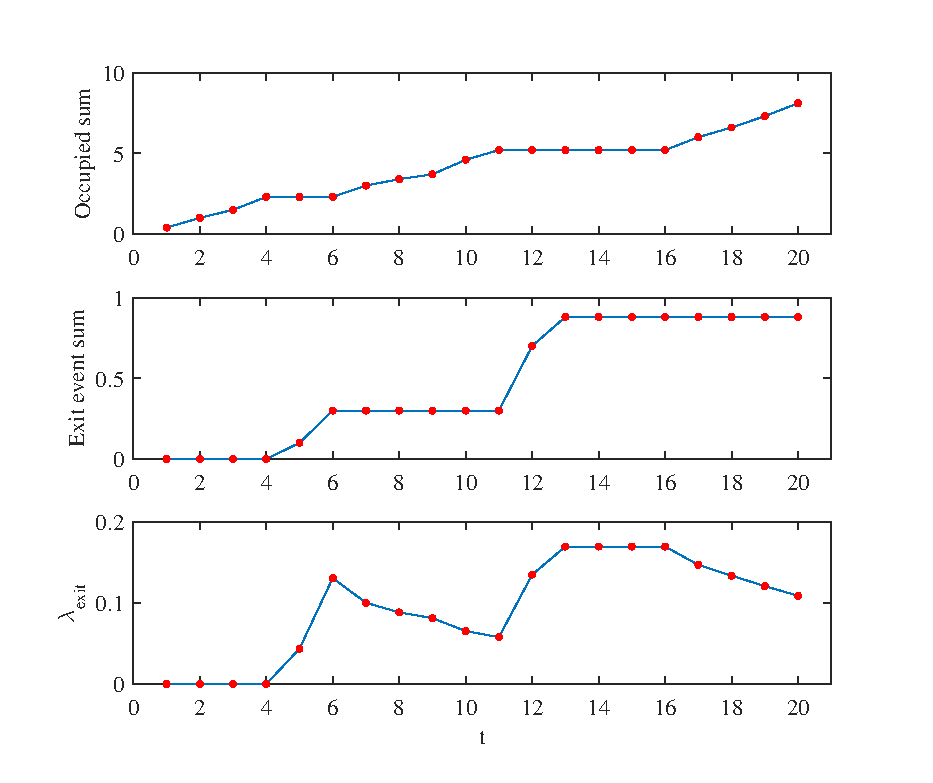
\includegraphics[scale=1]{chapters/mapping_of_dynamic_areas/figures/pmac_exit_explained}
\caption{Evolution of parameters used to estimate dynamics with the data shown in figure \ref{fig:state_scores_explained}.}
\label{fig:pmac_exit_explained}
\end{figure}

The observations from index $7$ to $20$ constitutes more certain changes in the state and thus carry more information which can be seen in the sums of especially the free score and entry event score. 

\begin{figure}[htbp]
    \centering
    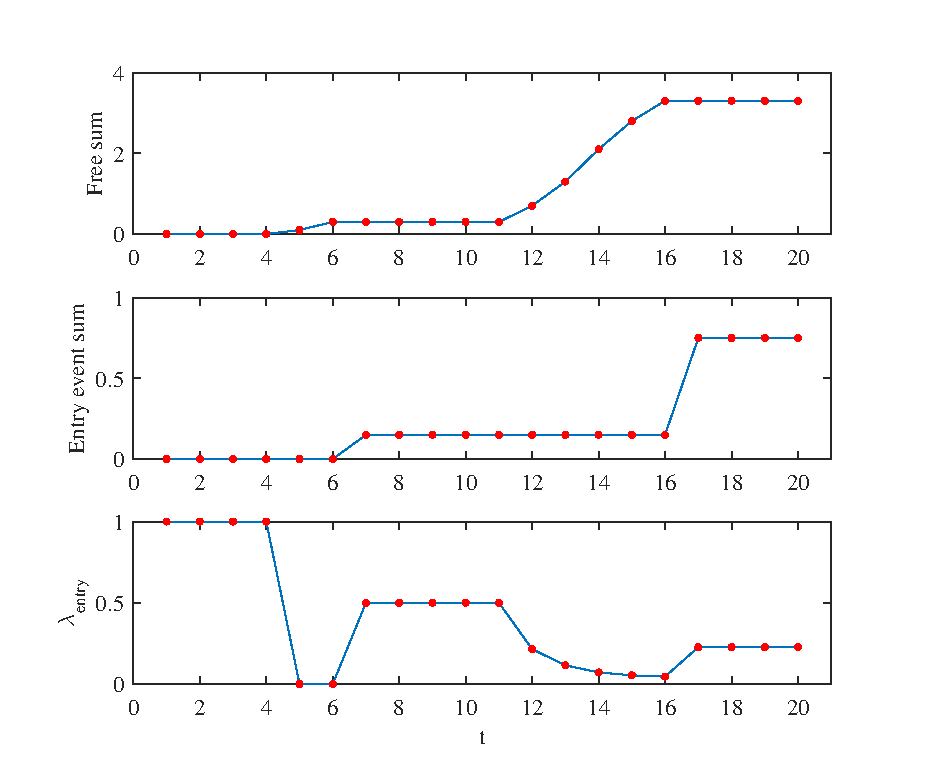
\includegraphics[scale=1]{chapters/mapping_of_dynamic_areas/figures/pmac_entry_explained}
    \caption{Evolution of parameters used to estimate dynamics with the data shown in figure \ref{fig:state_scores_explained}.}
    \label{fig:pmac_entry_explained}
\end{figure}


\subsection{Comparing PMAC to Alternavtives}
The goal of the developed PMAC learning method is to combine the fast learning under good condition from IMAC while also incorporating the uncertainty of sensor measurements. The uncertainty is represented as a probability from the static mapper that a cell is occupied. In order to compare PMAC to different Markov parameter learning methods, it has been tested in a simulation setup alongside IMAC and the online version of HMM. The test setup is one dimensional and a static mapper is used. The static mapper receives 10 noisy measurements, and determines the resulting occupancy probability as learning input. The simulation is run for 200 learning rounds with the noise changing midway through. The initial noise is \(1.2\) grid cells then decreasing to \(0.11\) grid cells, both with zero mean. 

The result of simulation run is shown in figure \ref{fig:markow_learning_pmac_comparison_entry} and \ref{fig:markow_learning_pmac_comparison_exit}. Figure  \ref{fig:markow_learning_pmac_comparison_entry} shows the learning of the \(p_{entry}\) parameter. It is clear that all of the methods has difficulties learning the correct value. But after observation number 100, and the decrease in noise, both IMAC and PMAC increases towards the correct value, with PMAC catching up to IMAC. All the methods underestimate the \(p_{entry}\).

\begin{figure}[H]
	\centering
	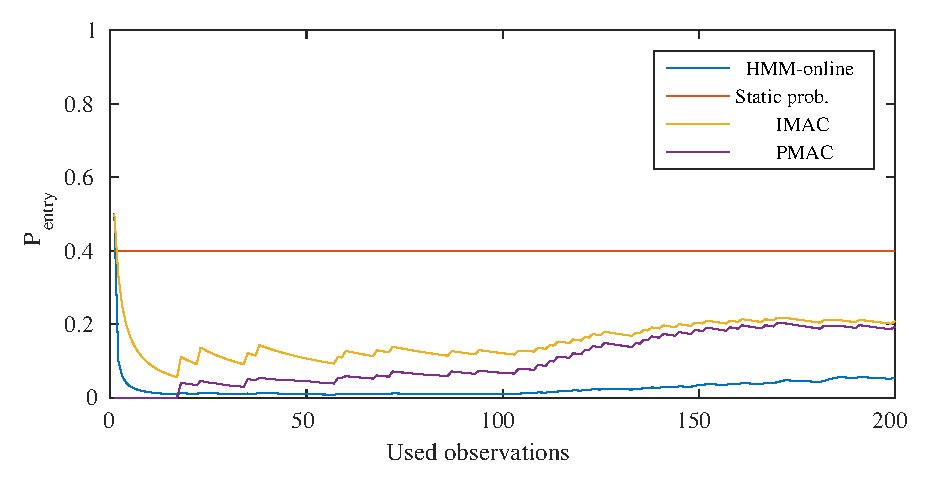
\includegraphics[scale=1]{chapters/mapping_of_dynamic_areas/figures/pmac_imac_hmm_entry}
	\caption{Estimated \(P_{entry}\) values for different learners}
	\label{fig:markow_learning_pmac_comparison_entry}
\end{figure}

The learning curves for \(P_{exit}\) is shown in figure \ref{fig:markow_learning_pmac_comparison_exit}. 
It is seen that \(P_{exit}\) is overestimated for the majority of the simulation. 
At observation number 100 it is seen that the decrease in noise has a significant effect on the estimates. 
PMAC experiences the most significant change when the noise changes. 
In the simulation shown the PMAC achieves the best result in estimating the \(P_{exit}\), but this is not consistently observed throughout all runs of the simulation. 
When the number of inputs, used in the static mapper before inputting to the learners, increases the difference between IMAC and PMAC becomes smaller as the static becomes increasingly certain on its output. 

\begin{figure}[H]
	\centering
	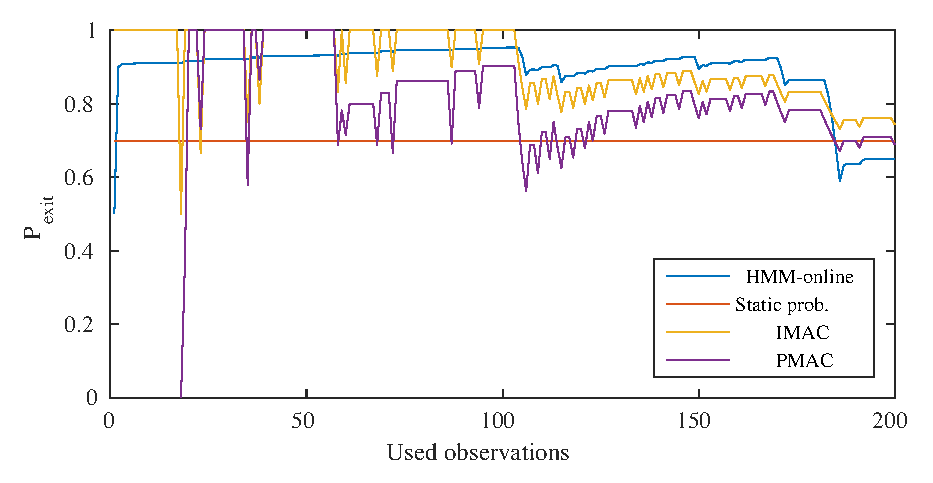
\includegraphics[scale=1]{chapters/mapping_of_dynamic_areas/figures/pmac_imac_hmm_exit}
	\caption{Estimated \(P_{exit}\) values for different learners}
	\label{fig:markow_learning_pmac_comparison_exit}
\end{figure}

The simulation shows that the ability of PMAC to learn the Markov parameters is at least comparable to the other learners when used with a static mapper. It is also observed that the static mapper increases IMAC's capability to handle zero-mean noise.
Despite not showing a vastly superior performance in the simulation, PMAC is chosen due to its abilities the handle various levels of certainty in observations. 

\subsection{Initializing the Dynamic Map}
As the dynamic map is the result of a learning process it will not contain any information from the onset. 
This might be a problem if the localization and navigation systems relies on the map to perform their tasks.
To handle this and guide the dynamic map it is possible to initialize the PMAC parameters. 
This could be done with the previously learned or a static map.
The initialization value of the PMAC parameters should be set according to the desired output and the confidence in the initial map.
If the confidence in the initial map is high then initializing with strong values helps to ensure that small errors will have less effect.